\documentclass{article}

% if you need to pass options to natbib, use, e.g.:
%     \PassOptionsToPackage{numbers, compress}{natbib}
% before loading neurips_2021

% ready for submission
\usepackage[preprint]{neurips_2021}

\setlength\intextsep{0mm}

%\usepackage{neurips_2021}

% to compile a preprint version, e.g., for submission to arXiv, add add the
% [preprint] option:
%     \usepackage[preprint]{neurips_2021}

% to compile a camera-ready version, add the [final] option, e.g.:
%     \usepackage[final]{neurips_2021}

% to avoid loading the natbib package, add option nonatbib:
%    \usepackage[nonatbib]{neurips_2021}

\usepackage[utf8]{inputenc} % allow utf-8 input
\usepackage[T1]{fontenc}    % use 8-bit T1 fonts
\usepackage{hyperref}       % hyperlinks
\usepackage{url}            % simple URL typesetting
\usepackage{booktabs}       % professional-quality tables
\usepackage{amsfonts}       % blackboard math symbols
\usepackage{nicefrac}       % compact symbols for 1/2, etc.
\usepackage{microtype}      % microtypography
\usepackage{xcolor}         % colors
\usepackage{graphicx}
\usepackage{array, booktabs, caption}
\usepackage{algorithm}
\usepackage{algpseudocode}

\title{Analysis of BERT and LSTM Based Models on Multi-label Coding Questions Classification}

% The \author macro works with any number of authors. There are two commands
% used to separate the names and addresses of multiple authors: \And and \AND.
%
% Using \And between authors leaves it to LaTeX to determine where to break the
% lines. Using \AND forces a line break at that point. So, if LaTeX puts 3 of 4
% authors names on the first line, and the last on the second line, try using
% \AND instead of \And before the third author name.

\author{%
  Tianle Wang \\
  Department of Computer Science\\
  University of Toronto\\
  \texttt{tianle.wang@mail.utoronto.ca} \\
  \And Yifan Zhao \\
  Department of Computer Science\\ 
  University of Toronto\\
  \texttt{ethany.zhao@mail.utoronto.ca} \\
  \And Yuezhexuan Zhu \\
  Department of Computer Science\\
  University of Toronto\\
  \texttt{yuezhexuan.zhu@mail.utoronto.ca} \\
}

\begin{document}

\maketitle
\begin{abstract}
Inspired by the neural language models introduced in the lecture, we have decided to design a neural network that can predict the labels of algorithms and data structures required to solve a coding question. To accomplish this, we have chosen to utilize the problems from \href{https://leetcode.com/}{Leetcode}. With relatively small data-set size, we use techniques including data augmentation and transfer learning to improve model performance. Our goal is to create a model that can predict the most likely algorithm for a given coding question based on its text description. 

For this project, we have structured two models on the basis of BERT\cite{BERT} and LSTM\cite{LSTM} along with specialized fine-tunings. Our analysis shows that BERT performs better than LSTM, and has potential for achieving higher accuracy. 

All related documents and data can be found inside our github repository\footnote{Github Link \href{https://github.com/XFTTech/CSC413-Project}{here}}.
\end{abstract}
\section{Introduction}
All members of our team share a common interest in solving coding questions, which we perceive as a means of enhancing our logical reasoning and programming proficiency. We have observed that the identification of an appropriate algorithm constitutes the initial and crucial step towards devising a solution. Any biased identification can lead to a series of fruitless tries until the correct algorithm is identified.

To address this issue, we aim at designing a Neural Network that can effectively generate potential algorithms and data structure labels for a given coding question based on its textual description. Our proposed model would take a coding question description and predict data structure and algorithm labels that feature in real solutions.

After selection and feasibility analysis, we decided to build our model on the basis of BERT\cite{BERT}, a multi-purpose transformer architecture, and LSTM\cite{LSTM}, a classic model for sequence classification. 
% While there exists a plethora of prior research and frameworks for these two models, we conduct data preprocessing, model designing, and several steps of architecture-specific embedding design and fine-tuning for developing a best-fit structure for multi-label coding question classification, where we will specify in detail along with conclusions in following sections.

% The existence of a plethora of prior research and frameworks allows us to analyze various architectures and leverage pre-trained models to minimize the resources required for training while achieving superior performance. Secondly, our model seeks to enhance the accuracy and efficiency of algorithm identification, thereby facilitating the solution development process.

\section{Data Preprocessing}
Instead of fetching data from Leetcode, we decide to use the processed dataset from gzipChrist\cite{DATA} on \href{https://www.kaggle.com/}{Kaggle}. The dataset comprises 1825 problem descriptions and their corresponding required algorithms or data structures. To facilitate analysis, we developed a Python script to vectorize the labels associated with each problem. Following processing, the dataset contains 1825 rows and 44 column, some of the processed data are shown in Table \ref{table:dataP}. The first column representing the problem description and the remaining columns indicating the presence or absence of the corresponding labels, denoted by binary values of 0 or 1. There are 43 labels in total.

\begin{table}[!h]
\centering
\caption{\textbf{Data After Processing}}
\begin{tabular}{ l c c c c c c c }
\toprule
% \hline
\textbf{Description} & \textbf{Array} & \textbf{DP} & \textbf{String} & \textbf{Math} & \textbf{$\cdots$} & \textbf{Hash Table} & \textbf{$\cdots$}  \\ 
\midrule
% \hline
Given an array of integers $\ldots$ & 1 & 0 & 0 & 0 & $\cdots$ & 1 & $\cdots$\\ 
% \hline
You are given two non-empty $\ldots$ & 0 & 0 & 0 & 1 & $\cdots$ & 0 & $\cdots$ \\
% \hline
$\cdots$ & $\cdots$ & $\cdots$ & $\cdots$ & $\cdots$ & $\cdots$ & $\cdots$ & $\cdots$\\
% \hline
\bottomrule
\end{tabular}
\label{table:dataP}
\end{table}

\section{Model Architecture}

\subsection{BERT Pre-trained Model}
\subsubsection{General Design}
On the basis of BERT, we selected the pre-trained CodeBERT\cite{CodeBERT} model and its corresponding tokenizer due to its relevance towards coding. Since there's a mismatch between BERT output and target labels counts, we added two extra fully connected layers to reduce output dimension to 43.
\begin{algorithm}
\caption{Forward Propagation Route}\label{alg:cap}
\begin{algorithmic}[1]
\State Input $\gets$ \texttt{Translate(Input, en$\to$ rand$\to$ en)} \Comment{Data Augmentation}
\State Input, Mask $\gets$ \texttt{tokenizer.encode(Input)} \Comment{Input Encoding}
\State Mid1 $\gets$ \texttt{CodeBERT(Input, Mask)} \Comment{BERT Layer}
\State Mid2 $\gets$ \texttt{Linear(Mid1, 768 $\to$ 512)} \Comment{FC \#1}
\State Mid3 $\gets$ \texttt{Linear(ReLU(Mid2), 512 $\to$ 43)} \Comment{FC \#2}
\State Output $\gets$ \texttt{Sigmoid(Mid3)} \Comment{Final Activation}
\end{algorithmic}
\end{algorithm}

Considering the fact that each description has more than one label, we first use the sigmoid function to regularization outputs and then apply binary cross-entropy loss as a loss function.

Through several rounds of tuning, we use $2\times 10^{-5}$ for the learning rate, $8$ as the batch size for data loader, Adam for optimizer with weight decay of $0.01$, and set the epoch to be $30$.
\begin{algorithm}
\caption{Single Training Step}\label{alg:cap}
\begin{algorithmic}[1]
\For{data in Dataloader}:
\State input, target $\gets$ data
\State output $\gets$ \texttt{model(input)}
\State loss $\gets$ \texttt{BCELoss(output, target)} \Comment{Binary Cross-Entropy Loss}
\State loss.backward() \Comment{Pytorch Function}
\State Adam.step() \Comment{Optimizer Step}
\State Adam.zero\_grad()
\EndFor
\end{algorithmic}
\end{algorithm}
\subsubsection{Input Encoding}
1825 inputs are less than the ideal amount, so we perform data augmentation on the dataset loader by translating loaded problem descriptions to a randomly selected language and then back to English before tokenizing the text, which is referred to in the algorithm box above.

As shown in histogram\ref{fig:len_hist}, as most descriptions in range from 50 to 400 characters, we use 512 as the maximum length for input encoding.

% \begin{figure}[h!]
%     \centering
%     \includegraphics[width = 0.45\textwidth]{img/distribution_input_length.png}
%     \caption{Distribution of input length}
%     \label{fig:distribution_length}
% \end{figure}

\subsubsection{Validation \& Analysis}
For calculating validation accuracy, we convert the predicted tensor to binary form using $0.5$ as threshold and employed \href{https://scikit-learn.org/stable/modules/generated/sklearn.metrics.accuracy_score.html}{\texttt{sklearn.metrics.accuracy\_score}} to get the accuracy score, which basically evaluates the percentage of complete matches between prediction and target. Then, we recorded the loss for both training and validation and accuracy for validation, with results shown in Figure \ref{fig:bert_plot}.

% While the raw accuracy of arbitrarily picking one label from 43 labels, it has a ${\displaystyle \frac{1}{43}=0.023}$ probability for picking the correct one, whereas the best validation accuracy of our model reaches $0.24$ at epoch 14, a substantial improvement.

% Other than testing complete matching, we continued on calculating label-wise matching accuracy between prediction and target, where we get $0.9520$ on reserved test set - an average of $2.064$ different labels overall, which can be either from prediction labels that don't exist or missing actual labels.

% Therefore, in overall, BERT models results are satisfying, and we'll turn to LSTM for further comparison.
In comparison to the random selection of one label from a pool of $43$, which yields a probability of ${\displaystyle \frac{1}{43}=0.023}$ for choosing the correct label, our model demonstrates a significant enhancement, achieving a peak validation accuracy of $0.24$ at epoch $14$. 

In addition to evaluating complete matching, we proceeded to compute the label-wise matching accuracy between predictions and targets. Our analysis revealed a \textbf{0.9632} accuracy on the reserved test set, with an average discrepancy of 1.582 labels overall. This discrepancy may arise from predicted labels that do not exist or from the omission of actual labels. In conclusion, the BERT model’s performance is satisfactory, and we will proceed to examine LSTM models for further comparison.

\begin{figure}[h!]
    \centering
    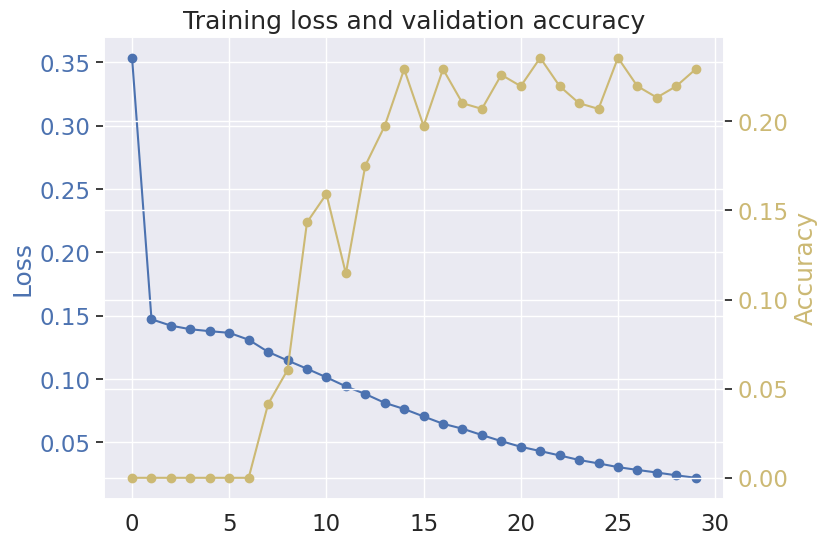
\includegraphics[width = 0.45\textwidth]{img/bert_train_plot.png}
    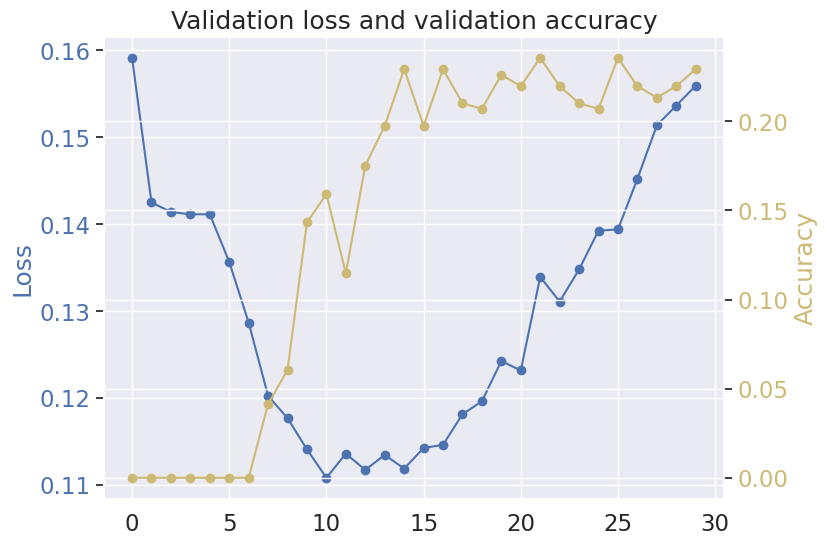
\includegraphics[width = 0.45\textwidth]{img/bert_val_plot.png}
    \caption{BERT train loss V.S. Epoch, validation loss V.S. Epoch and Accuracy V.S Epoch}
    \label{fig:bert_plot}
\end{figure}

\subsection{LSTM Model}
\subsubsection{General Design}
% To enable model training, we need to convert our input word sentences into vectors. We use \href{https://www.tensorflow.org/api_docs/python/tf/keras/preprocessing/text/Tokenizer}{\texttt{keras.preprocessing.text.Tokenizer}} as the tool to process our inputs. In an LSTM (Long Short-Term Memory) model, the input sequences must have a fixed length to be efficiently processed by the model. Therefore, we select the maximum length of the tokenized inputs as the target length and pad the other inputs to that length.

% Our model will embed the input and process its output using an LSTM layer. To regularize the outputs, we will apply a sigmoid function, and the binary cross-entropy loss function will be used to measure the difference between the predicted and actual outputs.
In order to facilitate model training, it is essential to transform the input word sentences into vector representations. The tool employed for this purpose is the \href{https://www.tensorflow.org/api_docs/python/tf/keras/preprocessing/text/Tokenizer}{\texttt{keras.preprocessing.text.Tokenizer}}. Within the context of an LSTM\cite{LSTM} model, input sequences necessitate a fixed length to ensure efficient processing. Consequently, the maximum length of tokenized inputs is chosen as the target length, and the remaining inputs are padded accordingly.

The proposed model will incorporate an embedding layer for the input and utilize an LSTM layer for processing the output. To achieve regularization of the outputs, a sigmoid function will be applied. Furthermore, the binary cross-entropy loss function will be employed to quantify the discrepancy between the predicted and actual outputs.

Through several rounds of tuning, we use $2\times 10^{-5}$ for the learning rate, 128 units for LSTM layer, maximum description length as the padding length, 32 for batch size, Adam for the optimizer with weight decay of $0.01$, and set the epoch to be $60$.
\begin{algorithm}
\caption{Forward Propagation Route}\label{alg:cap}
\begin{algorithmic}[1]
\State Input $\gets$ \texttt{Translate(Input, en$\to$ rand$\to$ en)} \Comment{Data Augmentation}
\State Input $\gets$ \texttt{tokenizer.encode(Input)} \Comment{Input Encoding}
\State Mid1 $\gets$ \texttt{LSTM(input, unit=128)} \Comment{LSTM Layer}
\State Mid2 $\gets$ \texttt{Linear(Mid1, $128\to 43$)} \Comment{Dense Layer}
\State Output $\gets$ \texttt{Sigmoid(Mid2)} \Comment{Final Activation}
\State
\State Model Fitting by Tensorflow:
\State \texttt{mode.fit(X, y, epochs=60, batch\_size=32, validation\_split=0.2)}
\end{algorithmic}
\end{algorithm}

\subsubsection{Training \& Validation}

For the purpose of comparison, we use the same schema as the BERT model, results are shown in Figure \ref{fig:lstm_plot}.
Recall the raw accuracy of arbitrarily picking one correct label with probability ${\displaystyle \frac{1}{43}=0.023}$, the LSTM model shown best validation accuracy of our model reaches $0.138$ at epoch 57 also a noticeable improvement. Same as the BERT model, we calculated label-wise matching accuracy between prediction and target, where we get $0.9470$ on the reserved test set - an average of $2.279$ for different labels overall, which can be either from prediction labels that don't exist or missing actual labels.

\begin{figure}[h!]
    \centering
    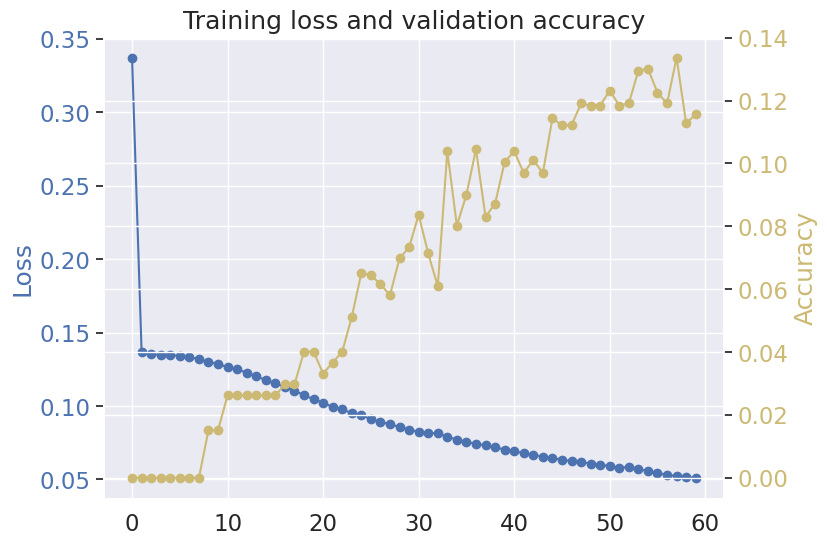
\includegraphics[width = 0.45\textwidth]{img/LSTM_train_plot.png}
    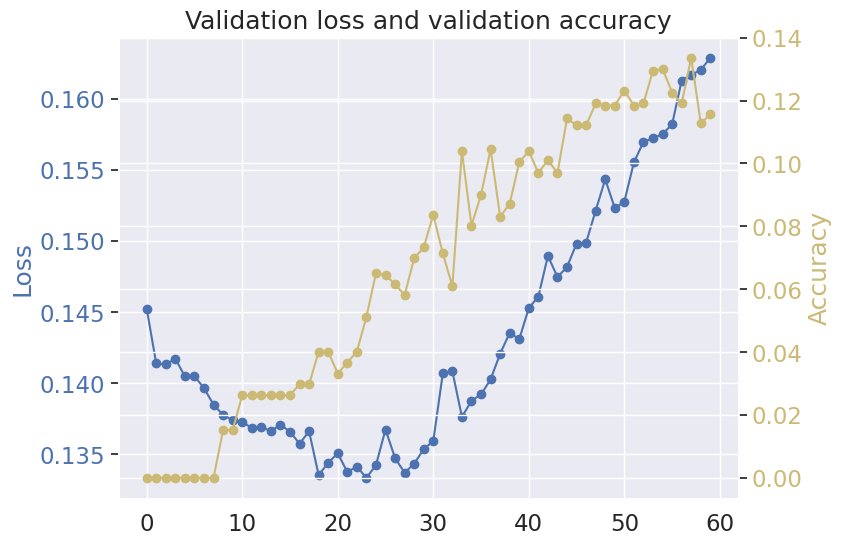
\includegraphics[width = 0.45\textwidth]{img/LSTM_val_plot.png}
    \caption{LSTM train loss V.S. Epoch, validation loss V.S. Epoch and Accuracy V.S Epoch}
    \label{fig:lstm_plot}
\end{figure}
\section{Comparison of Models}
In the realm of multi-label text classification, our experiment demonstrated superior performance by BERT, and in case of having sufficient computational resources, BERT proves to be the prior choice. Specifically, BERT has advantage over three aspects:

First, BERT model achieved a 0.24 validation accuracy rate, surpassing the LSTM model’s 0.138. Furthermore, both BERT and LSTM exhibited comparable label-wise accuracy rates of 0.9632 and 0.9470, respectively. This outcome may be attributed to BERT’s ability to effectively capture contextual information through its attention mechanism, while LSTMs potentially struggle with extended text sequences. 

Second, BERT's validation accuracy converges around epoch 15, while LSTM maintains an increasing trend till epoch 55. So, despite BERT having more per-epoch training costs, it converges faster.

Third, BERT outperforms LSTMs in handling out-of-vocabulary words due to its utilization of subword tokenization for addressing rare and unknown terms.
\section{Limitations}
In examining our dataset, several limitations must be acknowledged to ensure a comprehensive understanding of its potential impact on the analysis. 

Firstly, the dataset is relatively small. In particular, a small dataset may not provide enough information to enable models to learn the key relationships between words or phrases in the text to identify patterns effectively and generalize effectively to new data. 

Secondly, our model is limited to handling input from a text-based dataset (i.e. removing images from description), rendering it incapable of addressing problems that necessitate image understanding.

Thirdly, the labeling of LeetCode problems is inherently biased on associated with widely-used data structures and algorithms which indicates that the model's performance on non-Leetcode-like question-generation input and questions with uncommon algorithms may be significantly compromised.

Lastly, pre-trained tokenizers may separate formulas and characters from their associated words, making it difficult to learn relevant information from such text on certain topics. This can pose a challenge for our models that rely on tokenization to understand and process text data.
\section{Future Expectations}
With multiple online judging platforms, we may continue on tuning our model for a generalized coding question labeling network not limited to only Leetcode questions. 
Also, with BERT's strong competence, it's promising to further employ newly emerged models, including GPT and T5 to see if these models can reach human-level recognition. And, on the basis of using a pre-written tokenizer, a self-defined tokenizer and encoder may have the potential to further enhance model performance. 

%\section{Citations, figures, tables, references}
%\label{others}
%
%These instructions apply to everyone.
%
%\subsection{Citations within the text}
%
%The \verb+natbib+ package will be loaded for you by default.  Citations may be
%author/year or numeric, as long as you maintain internal consistency.  As to the
%format of the references themselves, any style is acceptable as long as it is
%used consistently.
%
%The documentation for \verb+natbib+ may be found at
%\begin{center}
%  \url{http://mirrors.ctan.org/macros/latex/contrib/natbib/natnotes.pdf}
%\end{center}
%Of note is the command \verb+\citet+, which produces citations appropriate for
%use in inline text.  For example,
%\begin{verbatim}
%   \citet{hasselmo} investigated\dots
%\end{verbatim}
%produces
%\begin{quote}
%  Hasselmo, et al.\ (1995) investigated\dots
%\end{quote}
%
%If you wish to load the \verb+natbib+ package with options, you may add the
%following before loading the \verb+neurips_2021+ package:
%\begin{verbatim}
%   \PassOptionsToPackage{options}{natbib}
%\end{verbatim}
%
%If \verb+natbib+ clashes with another package you load, you can add the optional
%argument \verb+nonatbib+ when loading the style file:
%\begin{verbatim}
%   \usepackage[nonatbib]{neurips_2021}
%\end{verbatim}
%
%As submission is double blind, refer to your own published work in the third
%person. That is, use ``In the previous work of Jones et al.\ [4],'' not ``In our
%previous work [4].'' If you cite your other papers that are not widely available
%(e.g., a journal paper under review), use anonymous author names in the
%citation, e.g., an author of the form ``A.\ Anonymous.''
%
%\subsection{Footnotes}
%
%Footnotes should be used sparingly.  If you do require a footnote, indicate
%footnotes with a number\footnote{Sample of the first footnote.} in the
%text. Place the footnotes at the bottom of the page on which they appear.
%Precede the footnote with a horizontal rule of 2~inches (12~picas).
%
%Note that footnotes are properly typeset \emph{after} punctuation
%marks.\footnote{As in this example.}
%
%\subsection{Figures}
%
%\begin{figure}
%  \centering
%  \fbox{\rule[-.5cm]{0cm}{4cm} \rule[-.5cm]{4cm}{0cm}}
%  \caption{Sample figure caption.}
%\end{figure}
%
%All artwork must be neat, clean, and legible. Lines should be dark enough for
%purposes of reproduction. The figure number and caption always appear after the
%figure. Place one line space before the figure caption and one line space after
%the figure. The figure caption should be lower case (except for first word and
%proper nouns); figures are numbered consecutively.
%
%You may use color figures.  However, it is best for the figure captions and the
%paper body to be legible if the paper is printed in either black/white or in
%color.
%
%\subsection{Tables}
%
%All tables must be centered, neat, clean and legible.  The table number and
%title always appear before the table.  See Table~\ref{sample-table}.
%
%Place one line space before the table title, one line space after the
%table title, and one line space after the table. The table title must
%be lower case (except for first word and proper nouns); tables are
%numbered consecutively.
%
%Note that publication-quality tables \emph{do not contain vertical rules.} We
%strongly suggest the use of the \verb+booktabs+ package, which allows for
%typesetting high-quality, professional tables:
%\begin{center}
%  \url{https://www.ctan.org/pkg/booktabs}
%\end{center}
%This package was used to typeset Table~\ref{sample-table}.
%
%\begin{table}
%  \caption{Sample table title}
%  \label{sample-table}
%  \centering
%  \begin{tabular}{lll}
%    \toprule
%    \multicolumn{2}{c}{Part}                   \\
%    \cmidrule(r){1-2}
%    Name     & Description     & Size ($\mu$m) \\
%    \midrule
%    Dendrite & Input terminal  & $\sim$100     \\
%    Axon     & Output terminal & $\sim$10      \\
%    Soma     & Cell body       & up to $10^6$  \\
%    \bottomrule
%  \end{tabular}
%\end{table}
%
%\section{Final instructions}
%
%Do not change any aspects of the formatting parameters in the style files.  In
%particular, do not modify the width or length of the rectangle the text should
%fit into, and do not change font sizes (except perhaps in the
%\textbf{References} section; see below). Please note that pages should be
%numbered.
%
%\section{Preparing PDF files}
%
%Please prepare submission files with paper size ``US Letter,'' and not, for
%example, ``A4.''
%
%Fonts were the main cause of problems in the past years. Your PDF file must only
%contain Type 1 or Embedded TrueType fonts. Here are a few instructions to
%achieve this.
%
%\begin{itemize}
%
%\item You should directly generate PDF files using \verb+pdflatex+.
%
%\item You can check which fonts a PDF files uses.  In Acrobat Reader, select the
%  menu Files$>$Document Properties$>$Fonts and select Show All Fonts. You can
%  also use the program \verb+pdffonts+ which comes with \verb+xpdf+ and is
%  available out-of-the-box on most Linux machines.
%
%\item The IEEE has recommendations for generating PDF files whose fonts are also
%  acceptable for NeurIPS. Please see
%  \url{http://www.emfield.org/icuwb2010/downloads/IEEE-PDF-SpecV32.pdf}
%
%\item \verb+xfig+ "patterned" shapes are implemented with bitmap fonts.  Use
%  "solid" shapes instead.
%
%\item The \verb+\bbold+ package almost always uses bitmap fonts.  You should use
%  the equivalent AMS Fonts:
%\begin{verbatim}
%   \usepackage{amsfonts}
%\end{verbatim}
%followed by, e.g., \verb+\mathbb{R}+, \verb+\mathbb{N}+, or \verb+\mathbb{C}+
%for $\mathbb{R}$, $\mathbb{N}$ or $\mathbb{C}$.  You can also use the following
%workaround for reals, natural and complex:
%\begin{verbatim}
%   \newcommand{\RR}{I\!\!R} %real numbers
%   \newcommand{\Nat}{I\!\!N} %natural numbers
%   \newcommand{\CC}{I\!\!\!\!C} %complex numbers
%\end{verbatim}
%Note that \verb+amsfonts+ is automatically loaded by the \verb+amssymb+ package.
%
%\end{itemize}
%
%If your file contains type 3 fonts or non embedded TrueType fonts, we will ask
%you to fix it.
%
%\subsection{Margins in \LaTeX{}}
%
%Most of the margin problems come from figures positioned by hand using
%\verb+\special+ or other commands. We suggest using the command
%\verb+\includegraphics+ from the \verb+graphicx+ package. Always specify the
%figure width as a multiple of the line width as in the example below:
%\begin{verbatim}
%   \usepackage[pdftex]{graphicx} ...
%   \includegraphics[width=0.8\linewidth]{myfile.pdf}
%\end{verbatim}
%See Section 4.4 in the graphics bundle documentation
%(\url{http://mirrors.ctan.org/macros/latex/required/graphics/grfguide.pdf})
%
%A number of width problems arise when \LaTeX{} cannot properly hyphenate a
%line. Please give LaTeX hyphenation hints using the \verb+\-+ command when
%necessary.
%
%\begin{ack}
%Use unnumbered first level headings for the acknowledgments. All acknowledgments
%go at the end of the paper before the list of references. Moreover, you are required to declare
%funding (financial activities supporting the submitted work) and competing interests (related financial activities outside the submitted work).
%More information about this disclosure can be found at: \url{https://neurips.cc/Conferences/2021/PaperInformation/FundingDisclosure}.
%
%Do {\bf not} include this section in the anonymized submission, only in the final paper. You can use the \texttt{ack} environment provided in the style file to autmoatically hide this section in the anonymized submission.
%\end{ack}

%\section*{References}
{
\small
\bibliographystyle{plain}
\begin{thebibliography}{9}
\bibitem{BERT}
Devlin, J., Chang, M., Lee, K., \& Toutanova, K. (2018). BERT: Pre-training of Deep Bidirectional Transformers for Language Understanding. ArXiv. /abs/1810.04805.
\bibitem{LSTM}
S. Hochreiter and J. Schmidhuber, "Long Short-Term Memory," in Neural Computation, vol. 9, no. 8, pp. 1735-1780, 15 Nov. 1997, doi: 10.1162/neco.1997.9.8.1735.
\bibitem{DATA}
gzipChrist. (2023, February). Leetcode Problem Dataset, Version 8.82. Retrieved April 10, 2023 from https://www.kaggle.com/datasets/gzipchrist/leetcode-problem-dataset.
\bibitem{CodeBERT}
Feng, Z., Guo, D., Tang, D., Duan, N., Feng, X., Gong, M., Shou, L., Qin, B., Liu, T., Jiang, D., \& Zhou, M. (2020). CodeBERT: A Pre-Trained Model for Programming and Natural Languages. ArXiv. /abs/2002.08155
\end{thebibliography}
}
%%%%%%%%%%%%%%%%%%%%%%%%%%%%%%%%%%%%%%%%%%%%%%%%%%%%%%%%%%%%
%\section*{Checklist}
%
%%%% BEGIN INSTRUCTIONS %%%
%The checklist follows the references.  Please
%read the checklist guidelines carefully for information on how to answer these
%questions.  For each question, change the default \answerTODO{} to \answerYes{},
%\answerNo{}, or \answerNA{}.  You are strongly encouraged to include a {\bf
%justification to your answer}, either by referencing the appropriate section of
%your paper or providing a brief inline description.  For example:
%\begin{itemize}
%  \item Did you include the license to the code and datasets? \answerYes{See Section~\ref{gen_inst}.}
%  \item Did you include the license to the code and datasets? \answerNo{The code and the data are proprietary.}
%  \item Did you include the license to the code and datasets? \answerNA{}
%\end{itemize}
%Please do not modify the questions and only use the provided macros for your
%answers.  Note that the Checklist section does not count towards the page
%limit.  In your paper, please delete this instructions block and only keep the
%Checklist section heading above along with the questions/answers below.
%%%% END INSTRUCTIONS %%%
%
%\begin{enumerate}
%
%\item For all authors...
%\begin{enumerate}
%  \item Do the main claims made in the abstract and introduction accurately reflect the paper's contributions and scope?
%    \answerTODO{}
%  \item Did you describe the limitations of your work?
%    \answerTODO{}
%  \item Did you discuss any potential negative societal impacts of your work?
%    \answerTODO{}
%  \item Have you read the ethics review guidelines and ensured that your paper conforms to them?
%    \answerTODO{}
%\end{enumerate}
%
%\item If you are including theoretical results...
%\begin{enumerate}
%  \item Did you state the full set of assumptions of all theoretical results?
%    \answerTODO{}
%	\item Did you include complete proofs of all theoretical results?
%    \answerTODO{}
%\end{enumerate}
%
%\item If you ran experiments...
%\begin{enumerate}
%  \item Did you include the code, data, and instructions needed to reproduce the main experimental results (either in the supplemental material or as a URL)?
%    \answerTODO{}
%  \item Did you specify all the training details (e.g., data splits, hyperparameters, how they were chosen)?
%    \answerTODO{}
%	\item Did you report error bars (e.g., with respect to the random seed after running experiments multiple times)?
%    \answerTODO{}
%	\item Did you include the total amount of compute and the type of resources used (e.g., type of GPUs, internal cluster, or cloud provider)?
%    \answerTODO{}
%\end{enumerate}
%
%\item If you are using existing assets (e.g., code, data, models) or curating/releasing new assets...
%\begin{enumerate}
%  \item If your work uses existing assets, did you cite the creators?
%    \answerTODO{}
%  \item Did you mention the license of the assets?
%    \answerTODO{}
%  \item Did you include any new assets either in the supplemental material or as a URL?
%    \answerTODO{}
%  \item Did you discuss whether and how consent was obtained from people whose data you're using/curating?
%    \answerTODO{}
%  \item Did you discuss whether the data you are using/curating contains personally identifiable information or offensive content?
%    \answerTODO{}
%\end{enumerate}
%
%\item If you used crowdsourcing or conducted research with human subjects...
%\begin{enumerate}
%  \item Did you include the full text of instructions given to participants and screenshots, if applicable?
%    \answerTODO{}
%  \item Did you describe any potential participant risks, with links to Institutional Review Board (IRB) approvals, if applicable?
%    \answerTODO{}
%  \item Did you include the estimated hourly wage paid to participants and the total amount spent on participant compensation?
%    \answerTODO{}
%\end{enumerate}
%
%\end{enumerate}

%%%%%%%%%%%%%%%%%%%%%%%%%%%%%%%%%%%%%%%%%%%%%%%%%%%%%%%%%%%%

\appendix

\section{Appendix}

Leetcode question description length histogram:
\begin{figure}[h!]
    \centering
    \includegraphics[width = 0.75\textwidth]{img/distribution_input_length.png}
    \caption{Input Length Distribution Histogram}
    \label{fig:len_hist}
\end{figure}

\end{document}
